\documentclass[../NFTComp_IEEE.tex]{subfiles}
\graphicspath{{\subfix{../Images}}}

\begin{document}
\section{Development of a NFT Smart Contract in Cadence}
\label{sec:cadence_development}
The approach in this section assumes a minimal knowledge from the reader about general blockchain technology and NFTs development in Solidity. As such, we opt to omit the implementation details from this blockchain and focus this text to the unfamiliar Cadence version. Fig. \ref{fig:cadence_nft_contract} presents a schematic representation of the contract developed displaying the required standard dependencies and the functions and fields required by this inheritance.

\begin{figure}[h!]
    \centering
    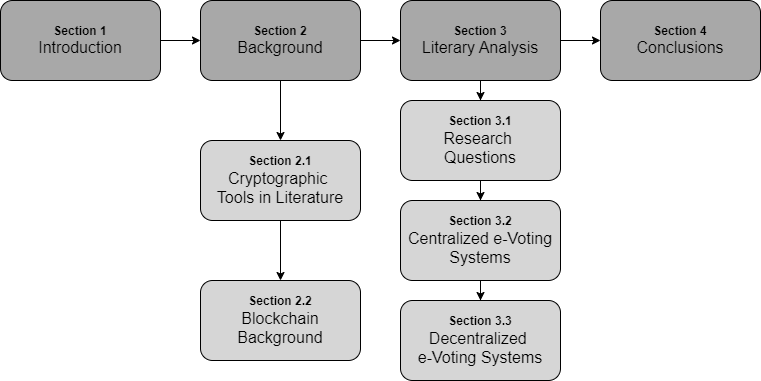
\includegraphics[width=\columnwidth]{Images/almei1.png}
    \caption{Structural organisation of a NFT smart contract in Cadence}
    \label{fig:cadence_nft_contract}
\end{figure}

\subsection{Standards Imported}
The simplest standardised version of a Cadence NFT smart contracts requires the import of two standards, namely, \textit{NonFungibleToken} and \textit{MetadataViews} interfaces. We omitted references to the \textit{MetadataViews} because this import is an imposition from the \textit{NonFungibleToken} import. Flow was developed towards supporting applications with high NFT throughput, such as digital collectibles for example. The \textit{MetadataViews} standard is used mostly to support metadata operations, which are used extensively in Flow to compose digital collectible objects similar to trading cards. This functional aspect falls outside the bounds of our study, so most of the requirements from this standard were ignored. We used a color scheme in Fig. \ref{fig:cadence_nft_contract} to indicate which standard required the function, resource and event indicated in the contract structure. The \textit{MetadataViews} requirements, since they are used to process token metadata, were implemented as stubs.

\subsubsection{Resources}
The \textit{NonFungibleToken} standard requires the implementation of NFT and a Collection resources as minimal requirements. But Fig. \ref{fig:cadence_nft_contract} shows a third resource in the contract, namely a \textit{NFTMinter}. This resource is used to abstract, simplify and secure the minting of new NFTs. New resources can only be created with a contract function due to Cadence restricting the "\textbf{create}" keyword to the context of the contract. Transactions are not able to invoke this internal action by themselves. The creation of new resources is restricted to contract functions. A secure and simple approach to resource creation is to define the create function inside of another resource and created and save it to owner account storage in the contract constructor. This restricts the creation of new NFTs to the owner of the account storage where the minter is saved, thus decoupling this action from the contract itself.

\subsubsection{Functions}
The \textit{NonFungibleToken} standard requires the implementation of a \textit{createEmptyCollection} function to obtain a collection resource, but it also requires similar implementations in the NFT and even in the collection resource itself. Standardised NFT contracts in Flow provide multiple access points to create new collections. The \textit{createEmptyCollection} function at the contract level requires a type as input because it is not possible to infer the storage type at that level. The versions at the resource level can infer the storage type by checking the type of the resource that is housing it.

\subsubsection{Events}
A contract that imports the \textit{NonFungibleToken} inherits the \textit{Withdrawn} and \textit{Deposited} events by default. In Cadence, like in Solidity, events are made available and emitted automatically by the logic imported from the standards, i.e., there is no need to define them explicitly in the contracts, unlike functions and resources. The events indicated are emitted automatically whenever a NFT resource is moved in or out of an account storage.
\end{document}